\chapter{Analýza}

\setcounter{page}{1}

\begin{chapterabstract}
V první podkapitole budu zkoumat podobné aplikace. V druhé podkapitole budu zkoumat zdrojová data, která budou použita pro přípravu dat na backendu pro použití mobilní aplikaci.
\end{chapterabstract}

\section{Podobné aplikace}
Popis podobných aplikaců

\subsection{politiscope}
Aplikace politiscope má za cíl poskytnout lidem informace ohledně politiky, a oheldně rozhodnutí zvolených politických reprezentantů ve Spojených Státech. Informace jsou objektivní a jsou lidem poskytovány v jednodušší formě, aby bylo lépe pochopitelné. Poskytuje shrnutí informací. Uživatelé mají možnost sledovat kategorie návrhů zákona  a konkrétního politika. Data vytahují z již existujících API, které povaýžují za věrohodné zdroje informací.

Informace jsou aktualizovány jednou denně. Články obsahují odkazy na články a videa relevantní k danému tématu. 

Témata zahrnuji návrhy zákonů, stav jejich schvalování, jejich souhrn. U návrhů jsou tagy pro jejich snazší filtrování a vyhledávání. Souhrny návrhů zákonů a odkaz na oficiální link oficiální webu Kongresu. Lze sledovat návrhy a politiky. Lze nastavit notifikaci. V době psaní práce má 10 000+ stahování.


\includegraphics[width=0.5\linewidth]{politiscope}

\subsection{Congress}
Aplikace Congress poskytuje informace o zvolených reprezentantech ve Spojených Státech, a jak hlasovali při schvalování zákonů. Lze vidět, které návrhy zákonů nás čekají. Lze hledat návrhy a výsledky hlasování. Lze nastavit notifikaci. Aplikace stahuje data z ProPublica's Conress API, který čerpá data z oficiálních stránek Kongresu.

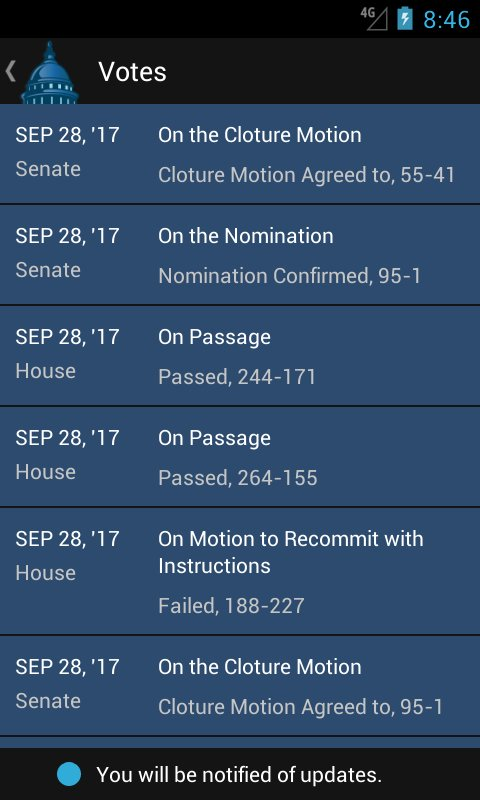
\includegraphics[width=0.5\linewidth]{congress}
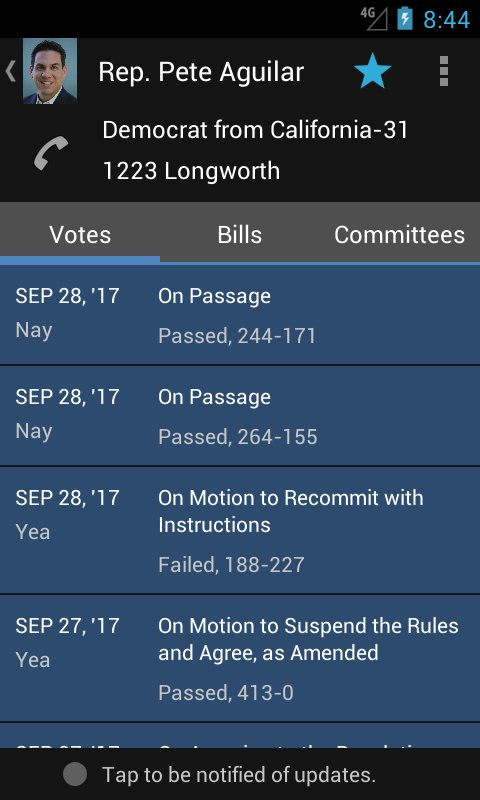
\includegraphics[width=0.5\linewidth]{congress-2}

\section{Zdrojová data}

\subsection{Zdroj}

Zdrojová data PS jsou volně ke stažení na https://www.psp.cz/sqw/hp.sqw?k=1300. Data jsou strukturovaná a pochází z agend PS a Senátu jako např. agenda poslanců, osob, hlasování a tisků. Pro účely této práce nás však budou zajímat pouze podmnožina dat agend z PS, které popíši později. 

\subsection{Formát dat}
Data jsou poskytována v souborech ve formátu UNL, tj.:

\begin{itemize}
	\item Každý řádek v souboru odpovídá jednom řádku v databázi.
	\item Oddělovačem je znak roury (|).
	\item Pokud je sloupec prázdný, je jeho hodnota typu null.
	\item V sloupcích jsou používány tzv. escape sekvence k zápisu speciálních znaků s úvodním znakem \ (backslash) následovaný znakem.
\end{itemize}

Tyto soubory jsou podle typu seskupeny do souborů ve formátu zip, např. poslanci.zip pro data o poslancích a hl-2021ps.zip pro data o hlasováních v 9. volebním období.

\subsection{Aktualizace}

Data obsahují úplný stav, rozdílové aktualizace nejsou poskytovány. To pro nás znamená, že při aktualizaci dat musíme rozdíly mezi zdrojovými daty a daty v databázi najít sami a podle toho aktualizovat databázi. Důležité při tom je to, aby data, která na sobě závisí, byla aktualizována tak, aby byla zaručena jejich konzistence. Tedy pokud při aktualizaci nějakého údaje musíme aktualizovat i všechny údaje, které na tom údaji závisí.

Pokud bude strunktura dat doplňována, budou nové sloupce přidávány na konec. Nové sloupce pro nás nebudou důležitá. Budeme pracovat pouze s daty, které tam jsou v době psaní diplomové práce.

\subsection{Kódování}
Kódování je windows-1250. Ten obsahuje mimo jiné všechny znaky z české abecedy. Na to bude potřeba brát ohled při ukládání dat do databáze, aby se toto kódování zachovalo.

\subsection{Datové typy}
Na stránce je uvedena tabulka obsahující typy dat sloupců v tabulkách a popis jejich významu.

\begin{longtable}{|l|p{9cm}|} \hline
	\multicolumn{2}{|l|}{\textbf{Typy dat sloupců v tabulkách}} \\ \hline
	\textbf{Typ} & \textbf{Popis} \\ \hline
	
	int	& integer \\ \hline
	
	char(X)		& textový řetězec, s blíže neuvedenou délkou
	 \\ \hline
	
	char(N)		& textový řetězec, s konktrétní délkou
	 \\ \hline	
	
	date	& datum, ve formátu DD.MM.YYYY
	 \\ \hline	
	 
 	datetime(year to hour)		& datum a čas, do úrovně hodin, ve formátu YYYY-MM-DD HH
 	
	 \\ \hline
	 
 	datetime(year to second)		& datum a čas, do úrovně vteřin, ve formátu YYYY-MM-DD HH:TT:SS
 	
	 \\ \hline
	 
 	datetime(..., fraction)		& Doplnění formátu o zlomky vteřiny, odděleno tečkou od původního formátu
 	
	 \\ \hline
	 
 	datetime(hour to minute)		& čas, ve formátu HH:MM
	 \\ \hline
	
	\caption{Typy dat sloupců v tabulkách}
	\label{table:data_types}
\end{longtable}

\subsection{Licence}

Data jsou poskytována bezplatně, využití dat je podmíněno uvedením zdroje dat a případně datem zpracování dat. Mobilní aplikace a backend budou implementovány ve dvou různých repozitářích. V každém z nich uvedeno, odkud data pocházela.

\subsection{Tabulky}

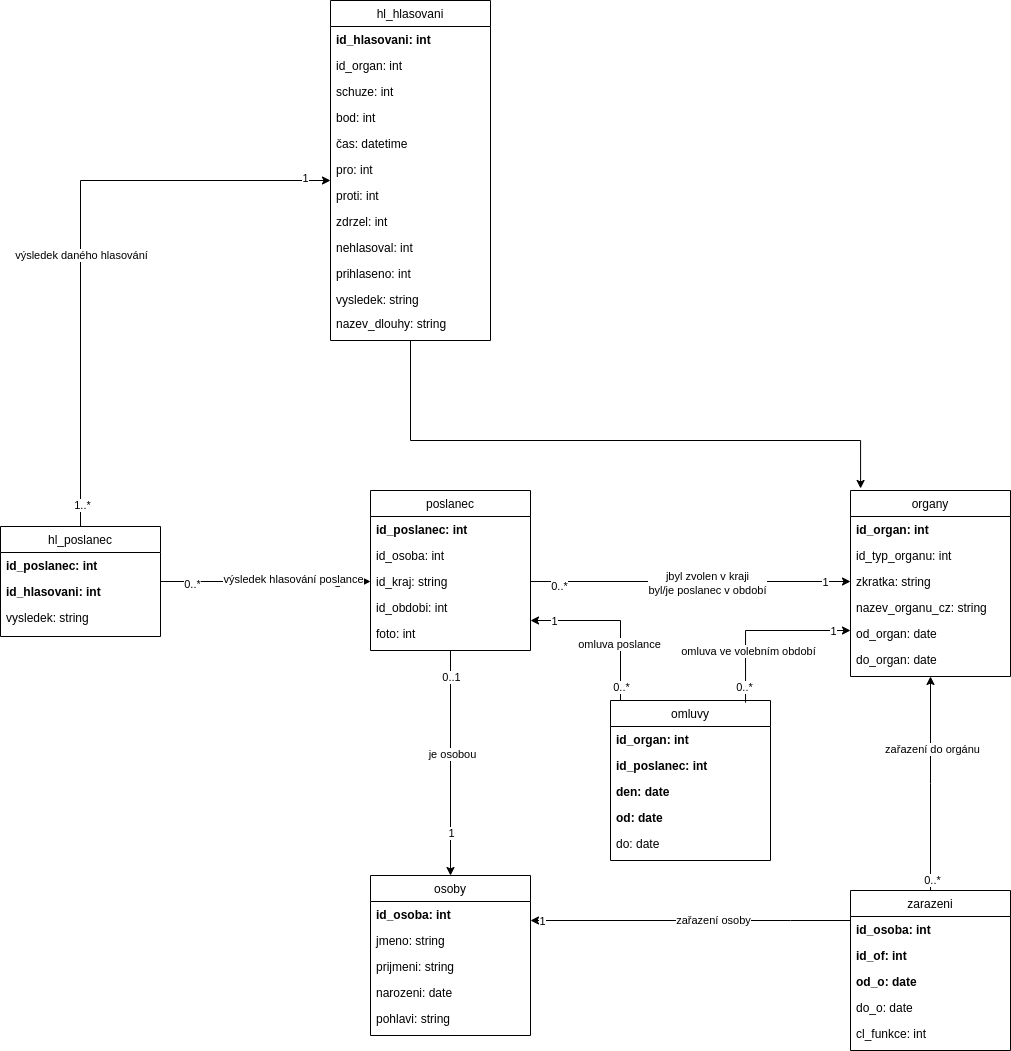
\includegraphics[width=\linewidth]{source_data_diagram}

\subsubsection{typ\textunderscore organu}

Orgány mají svůj typ, tyto typy mají hiearchickou strukturu.

\begin{center}
	\begin{longtable}{|l|l|p{9cm}|}
		\caption{Tabulka typ\textunderscore organu} \label{table:typ_organu} \\
		
		\hline 
		
		\multicolumn{3}{|l|}{\textbf{Tabulka typ\textunderscore organu}} \\
		
		\hline 
		
		\multicolumn{1}{|l|}{\textbf{Sloupec}} & \multicolumn{1}{l|}{\textbf{Typ}} & \multicolumn{1}{l|}{\textbf{Použití a vazby}} \\ 

		\endhead
		
		\hline 
		
		id\textunderscore typ\textunderscore org & int & Identifikátor typu orgánu \\
		
		\hline 
		
		typ\textunderscore id\textunderscore typ\textunderscore org	 org & int & Identifikátor nadřazeného typu orgánu (typ\textunderscore organu:id\textunderscore typ\textunderscore org), pokud je null či nevyplněno, pak nemá nadřazený typ \\
		
		\hline 
		
		nazev\textunderscore typ\textunderscore org\textunderscore cz & char(X) & Název typu orgánu v češtině \\
		
		\hline 
		
		nazev\textunderscore typ\textunderscore org\textunderscore en & char(X) & Název typu orgánu v angličtině \\
		
		\hline 
		
		typ\textunderscore org\textunderscore obecny & int & Obecný typ orgánu, pokud je vyplněný, odpovídá záznamu v typ\textunderscore organu:id\textunderscore typ\textunderscore org. Pomocí tohoto sloupce lze najít např. všechny výbory v různých typech zastupitelských sborů. \\
		
		\hline 
		
		priorita & int & Priorita při výpisu \\
		
		\hline 

	\end{longtable}
\end{center}

\subsubsection{organy}

Některé orgány mají nadřazený orgán a pak je položka organy:organ\textunderscore id\textunderscore organ vyplněna, přičemž pouze v některých případech se tyto vazby využívají.

\begin{center}
	\begin{longtable}{|l|l|p{9cm}|}
		\caption{Tabulka organy} \label{table:organy} \\
		
		\hline 
		
		\multicolumn{3}{|l|}{\textbf{Tabulka organy}} \\
		
		\hline 
		
		\multicolumn{1}{|l|}{\textbf{Sloupec}} & \multicolumn{1}{l|}{\textbf{Typ}} & \multicolumn{1}{l|}{\textbf{Použití a vazby}} \\ 
		
		\endhead
		
		\hline 
		
		id\textunderscore organ & int & Identifikátor orgánu \\
		
		\hline 
		
		organ\textunderscore id\textunderscore organ & int & Identifikátor nadřazeného orgánu, viz organy:id\textunderscore organ \\
		
		\hline 
		
		id\textunderscore typ\textunderscore organu & int & Typ orgánu, viz typ\textunderscore organu:id\textunderscore typ\textunderscore organu \\
		
		\hline 
		
		zkratka & char(X) & Zkratka orgánu, bez diakritiky, v některých připadech se zkratka při zobrazení nahrazuje jiným názvem \\
		
		\hline 
		
		nazev\textunderscore organu\textunderscore cz	 & char(X)	 & Název orgánu v češtině
		 \\
		
		\hline 
		
		nazev\textunderscore organu\textunderscore en	 & char(X)	 & Název orgánu v angličtině
		 \\
		
		\hline 
		
		od\textunderscore organ & date & Ustavení orgánu
		 \\
		
		\hline 
		
		do\textunderscore organ & date & Ukončení orgánu
		 \\
		
		\hline 
		
		priorita & int & Priorita výpisu orgánů
		 \\
		
		\hline 
		
		cl\textunderscore organ\textunderscore base	 & int & Pokud je nastaveno na 1, pak při výpisu členů se nezobrazují záznamy v tabulkce zarazeni kde cl\textunderscore funkce == 0. Toto chování odpovídá tomu, že v některých orgánech nejsou členové a teprve z nich se volí funkcionáři, ale přímo se volí do určité funkce. \\
		
		\hline 
		
	\end{longtable}
\end{center}

\subsubsection{osoby}

Obsahuje jména osob, které jsou zařazeni v orgánech. Vzhledem k tomu, že k jednoznačnému rozlišení osob často není dostatek informací, je možné, že ne všechny záznamy odkazují na jedinečné osoby, tj. některé osoby jsou v tabulce vícekrát.

\begin{center}
	\begin{longtable}{|l|l|p{9cm}|}
		\caption{Tabulka osoby
		} \label{table:osoby} \\
		
		\hline 
		
		\multicolumn{3}{|l|}{\textbf{Tabulka osoby
		}} \\
		
		\hline 
		
		\multicolumn{1}{|l|}{\textbf{Sloupec}} & \multicolumn{1}{l|}{\textbf{Typ}} & \multicolumn{1}{l|}{\textbf{Použití a vazby}} \\ 
		
		\endhead
		
		\hline 
		
		id\textunderscore osoba & int & Identifikátor osoby \\
		
		\hline 
		
		pred & char(X) & Titul pred jmenem \\
	
		\hline 
		
		jmeno & char(X) & Jméno \\
		
		\hline 
		
		prijmeni & char(X) & Příjmení, v některých případech obsahuje i dodatek typu "st.", "ml." \\
		
		\hline 
		
		za & char(X) & Titul za jménem \\
		
		\hline 
		
		narozeni & date & Datum narození, pokud neznámo, pak 1.1.1900. \\
		
		\hline 

		pohlavi & char(X) & Pohlaví, "M" jako muž, ostatní hodnoty žena \\
		
		\hline 
		
		zmena & date & Datum posledni změny \\
		
		\hline 
		
		umrti & date & Datum úmrtí \\
		
		\hline 
		
		
	\end{longtable}
\end{center}

\subsubsection{zarazeni}

Obsahuje data zařazení v orgánu nebo data funkcí osoby v orgánu. Pokud je zarazeni:do\textunderscore o typu null, pak jde o aktuální zařazení.

\begin{center}
	\begin{longtable}{|l|l|p{9cm}|}
		\caption{Tabulka zarazeni} 
		\label{table:zarazeni} \\
		
		\hline 
		
		\multicolumn{3}{|l|}{\textbf{Tabulka zarazeni}} \\
		
		\hline 
		
		\multicolumn{1}{|l|}{\textbf{Sloupec}} & \multicolumn{1}{l|}{\textbf{Typ}} & \multicolumn{1}{l|}{\textbf{Použití a vazby}} \\ 
		
		\endhead
		
		\hline 
		
		id\textunderscore osoba & int & Identifikátor osoby, viz osoba:id\textunderscore osoba \\
		
		\hline 
		
		id\textunderscore of & int & Identifikátor orgánu či funkce: pokud je zároveň nastaveno zarazeni:cl\textunderscore funkce == 0, pak id\textunderscore o odpovídá organy:id\textunderscore organ, pokud cl\textunderscore funkce == 1, pak odpovídá funkce:id\textunderscore funkce.
		 \\
		
		\hline 
		
		cl\textunderscore funkce & int & Status členství nebo funce: pokud je rovno 0, pak jde o členství, pokud 1, pak jde o funkci.
		 \\
		
		\hline 
		
		od\textunderscore o & datetime(year to hour)	 & Zařazení od
		 \\
		
		\hline 
		
		do\textunderscore o & datetime(year to hour)	 & Zařazení do
		 \\
		
		\hline 
		
		od\textunderscore f & date & Mandát od. Nemusí být vyplněno a pokud je vyplněno, pak určuje datum vzniku mandátu a zarazeni:od\textunderscore o obsahuje datum volby.
		 \\
		
		\hline 
		
		do\textunderscore f & date & Mandát do. Nemusí být vyplněno a pokud je vyplněno, určuje datum konce mandátu a zarazeni:do\textunderscore o obsahuje datum ukončení zařazení. \\
		
		\hline 
		
		
	\end{longtable}
\end{center}

\subsubsection{poslanec}

\begin{center}
	\begin{longtable}{|l|l|p{9cm}|}
		\caption{Tabulka poslanec} 
		\label{table:poslanec} \\
		
		\hline 
		
		\multicolumn{3}{|l|}{\textbf{Tabulka poslanec}} \\
		
		\hline 
		
		\multicolumn{1}{|l|}{\textbf{Sloupec}} & \multicolumn{1}{l|}{\textbf{Typ}} & \multicolumn{1}{l|}{\textbf{Použití a vazby}} \\ 
		
		\endhead
		
		\hline 
		
		id\textunderscore poslanec & int & Identifikátor poslance \\
		
		\hline 
		
		id\textunderscore osoba & int & Identifikátor osoby, viz osoba:id\textunderscore osoba \\
		
		\hline 
		
		id\textunderscore kraj & int & Volební kraj, viz organy:id\textunderscore organu \\
		
		\hline 
		
		id\textunderscore kandidatka & int & Volební strana/hnutí, viz org:id\textunderscore organu, pouze odkazuje na stranu/hnutí, za kterou byl zvolen a nemusí mít souvislost s členstvím v poslaneckém klubu. \\
		
		\hline 
		
		id\textunderscore obdobi & int & Volební období, viz organy:id\textunderscore organu \\
		
		\hline 
		
		web & char(X) & URL vlastních stránek poslance \\
		
		\hline 
		
		ulice & char(X) & Adresa regionální kanceláře, ulice. \\
		
		\hline 
		
		obec & char(X) & Adresa regionální kanceláře, obec. \\
		
		\hline 
		
		psc & char(X) & Adresa regionální kanceláře, PSČ. \\
		
		\hline 
		
		email & char(X) & E-mailová adresa poslance, případně obecná posta@psp.cz. \\
		
		\hline 
		
		telefon & char(X) & Adresa regionální kanceláře, telefon. \\
		
		\hline 
		
		fax & char(X) & Adresa regionální kanceláře, fax. \\
		
		\hline 
		
		psp\textunderscore telefon & char(X) & Telefonní číslo do kanceláře v budovách PS. \\
		
		\hline 
		
		facebook & char(X) & URL stránky služby Facebook. \\
		
		\hline 
		
		foto & int & Pokud je rovno 1, pak existuje fotografie poslance. \\
		
		\hline 
		
	\end{longtable}
\end{center}

\subsubsection{hl\textunderscore hlasovani}

\begin{center}
	\begin{longtable}{|l|l|p{9cm}|}
		\caption{Tabulka hl\textunderscore hlasovani} 
		\label{table:hl_hlasovani} \\
		
		\hline 
		
		\multicolumn{3}{|l|}{\textbf{Tabulka hl\textunderscore hlasovani}} \\
		
		\hline 
		
		\multicolumn{1}{|l|}{\textbf{Sloupec}} & \multicolumn{1}{l|}{\textbf{Typ}} & \multicolumn{1}{l|}{\textbf{Použití a vazby}} \\ 
		
		\endhead
		
		\hline 
		
		id\textunderscore hlasovani & int & Identifikátor hlasování \\
		
		\hline 
		
		id\textunderscore organ & int & Identifikátor orgánu, viz organy:id\textunderscore organ	 \\
		
		\hline 
		
		schuze & int & Číslo schůze
		 \\
		
		\hline 
		
		cislo & int & Číslo hlasování
		 \\
		
		\hline 
		
		bod & int & Bod pořadu schůze; je-li menší než 1, pak jde o procedurální hlasování nebo o hlasování k bodům, které v době hlasování neměly přiděleno číslo.
		 \\
		
		\hline 
		
		datum & date & Datum hlasování
		 \\
		
		\hline 
		
		čas & datetime(hour to minute)	 & Čas hlasování
		 \\
		
		\hline 
		
		pro & int & Počet hlasujících pro
		 \\
		
		\hline 
		
		proti & int & Počet hlasujících proti
		 \\
		
		\hline 
		
		zdrzel & int & Počet hlasujících zdržel se, tj. stiskl tlačítko X
		 \\
		
		\hline 
		
		nehlasoval & int & Počet přihlášených, kteří nestiskli žádné tlačítko
		 \\
		
		\hline 
		
		prihlaseno & int & Počet přihlášených poslanců
		 \\
		
		\hline 
		
		kvorum & int & Kvórum, nejmenší počet hlasů k přijetí návrhu
		 \\
		
		\hline 
		
		druh\textunderscore hlasovani & char(X)	 & Druh hlasování: N - normální, R - ruční (nejsou známy hlasování jednotlivých poslanců), E - vinou technické závady nejsou dostupná všechna data k hlasování, např. výsledky hlasování jednotlivých poslanců.
		 \\
		
		\hline 
		
		vysledek & char(X)	 & Výsledek: A - přijato, R - zamítnuto, jinak zmatečné hlasování
		 \\
		
		\hline 
		
		nazev\textunderscore dlouhy & char(X)	 & Dlouhý název bodu hlasování
		 \\
		
		\hline 
		
		nazev\textunderscore kratky & char(X)	 & Krátký název bodu hlasování \\
		
		\hline 
		
	\end{longtable}
\end{center}

\subsubsection{hl\textunderscore poslanec}

Tabulka zaznamenává výsledek hlasování jednotlivého poslance.

\begin{center}
	\begin{longtable}{|l|l|p{9cm}|}
		\caption{Tabulka hl\textunderscore poslanec} 
		\label{table:hl_hlasovani} \\
		
		\hline 
		
		\multicolumn{3}{|l|}{\textbf{Tabulka hl\textunderscore poslanec}} \\
		
		\hline 
		
		\multicolumn{1}{|l|}{\textbf{Sloupec}} & \multicolumn{1}{l|}{\textbf{Typ}} & \multicolumn{1}{l|}{\textbf{Použití a vazby}} \\ 
		
		\endhead
		
		\hline 
		
		id\textunderscore poslanec & int & Identifikátor poslance, viz poslanec:id\textunderscore poslanec
		 \\
		
		\hline 
		
		id\textunderscore hlasovani & int & Identifikátor hlasování, viz hl\textunderscore hlasovani:id\textunderscore hlasovani
		\\
		
		\hline 
		
		vysledek & char(X) & Hlasování jednotlivého poslance. 'A' - ano, 'B' nebo 'N' - ne, 'C' - zdržel se (stiskl tlačítko X), 'F' - nehlasoval (byl přihlášen, ale nestiskl žádné tlačítko), '@' - nepřihlášen, 'M' - omluven, 'W' - hlasování před složením slibu poslance, 'K' - zdržel se/nehlasoval. Viz úvodní vysvětlení zpracování výsledků hlasování.
		\\
		
		\hline 
		
	\end{longtable}
\end{center}

\subsubsection{omluvy}

Tabulka zaznamenává časové ohraničení omluv poslanců z jednání Poslanecké sněmovny.

\begin{center}
	\begin{longtable}{|l|l|p{9cm}|}
		\caption{Tabulka omluvy} 
		\label{table:omluvy} \\
		
		\hline 
		
		\multicolumn{3}{|l|}{\textbf{Tabulka omluvy}} \\
		
		\hline 
		
		\multicolumn{1}{|l|}{\textbf{Sloupec}} & \multicolumn{1}{l|}{\textbf{Typ}} & \multicolumn{1}{l|}{\textbf{Použití a vazby}} \\ 
		
		\endhead
		
		\hline 
		
		id\textunderscore organ & int & Identifikátor volebního období, viz organy:id\textunderscore organ
			\\
		
		\hline 
		
		id\textunderscore poslanec & int & Identifikátor poslance, viz poslanec:id\textunderscore poslanec
			\\
		
		\hline 
		
		
		den & date & Datum omluvy
			\\
		
		\hline 
		
		
		od & datetime(hour to minute)	 & Čas začátku omluvy, pokud je null, pak i omluvy:do je null a jedná se o omluvu na celý jednací den.
			\\
		
		\hline 
		
		
		do & datetime(hour to minute)	 & Čas konce omluvy, pokud je null, pak i omluvy:od je null a jedná se o omluvu na celý jednací den.	\\
		
		\hline 
		
	\end{longtable}
\end{center}






